\subsubsection{UC\theuccount-CT - Gestore Personale invia il messaggio finale al Consumer Telegram}
	\begin{figure}[H]
		\centering
		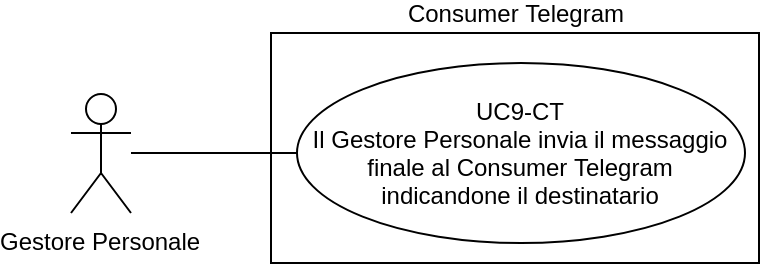
\includegraphics[width=0.6\textwidth]{img/casi_d'uso/UC9.png}\\
		\caption{UC\theuccount-CT - Gestore Personale invia il messaggio finale al Consumer Telegram}
	\end{figure}
	\begin{itemize}
		\item \textbf{Codice}: UC\theuccount-CT.
		\item \textbf{Titolo}: Gestore Personale invia il messaggio finale al Consumer Telegram.
		\item \textbf{Attori primari}: Gestore Personale.
		\item \textbf{Descrizione}: il Gestore Personale, dopo aver ricevuto il messaggio elaborato
		dai Producer Redmine o GitLab, controlla i messaggi sullo specifico Topic "commits", se ce ne
		sono vengono analizzati in base alla	lista di keyword. Se gli utenti iscritti a quella determinata
		keyword sono disponibili e se vogliono ricevere il messaggio tramite Telegram viene preparato
		il messaggio finale da inviare e inviato al Consumer Telegram. Altrimenti valuta il campo Topic del
		messaggio e controlla chi è iscritto a quel Topic, se gli utenti iscritti a quel Topic sono disponibili e
		se vogliono ricevere il messaggio tramite Telegram. Se tutte queste condizioni sono verificate, viene preparato
		il messaggio finale da inviare e inviato al Consumer Telegram.\\
		Il messaggio finale, una volta elaborato, conterrà i campi:
		\begin{itemize}
			\item Id della chat del destinatario
			\item Applicazione di provenienza
			\item Ora di invio
			\item Tipo di segnalazione(commit o issue)
			\item Project
			\item Topic
			\item Subject e opzionalmente
		 	\begin{itemize}
				\item Description
				\item Due date
				\item Milestone
				\item Assignee
			\end{itemize}
		\end{itemize}
		\item \textbf{Precondizione}: il Gestore Personale ha ricevuto il messaggio elaborato dai Producer Redmine o GitLab.
		\item \textbf{Postcondizione}: Il Gestore Personale ha inviato il messaggio finale al Consumer Telegram.
		\item \textbf{Scenario principale}: 
		\begin{enumerate}
			\item ll Gestore Personale riceve un messaggio dal Producer Redmine o dal Producer GitLab
			\item Il Gestore Personale valuta quali utenti sono iscritti al Topic del messaggio ricevuto, se sono disponibili e se vogliono ricevere il messaggio tramite Telegram
			\item Gestore Personale procede all'invio del messaggio finale al Consumer Telegram
		\end{enumerate}
		
	\end{itemize}